\documentclass{article}\usepackage[]{graphicx}\usepackage[]{color}
%% maxwidth is the original width if it is less than linewidth
%% otherwise use linewidth (to make sure the graphics do not exceed the margin)
\makeatletter
\def\maxwidth{ %
  \ifdim\Gin@nat@width>\linewidth
    \linewidth
  \else
    \Gin@nat@width
  \fi
}
\makeatother

\definecolor{fgcolor}{rgb}{0.345, 0.345, 0.345}
\newcommand{\hlnum}[1]{\textcolor[rgb]{0.686,0.059,0.569}{#1}}%
\newcommand{\hlstr}[1]{\textcolor[rgb]{0.192,0.494,0.8}{#1}}%
\newcommand{\hlcom}[1]{\textcolor[rgb]{0.678,0.584,0.686}{\textit{#1}}}%
\newcommand{\hlopt}[1]{\textcolor[rgb]{0,0,0}{#1}}%
\newcommand{\hlstd}[1]{\textcolor[rgb]{0.345,0.345,0.345}{#1}}%
\newcommand{\hlkwa}[1]{\textcolor[rgb]{0.161,0.373,0.58}{\textbf{#1}}}%
\newcommand{\hlkwb}[1]{\textcolor[rgb]{0.69,0.353,0.396}{#1}}%
\newcommand{\hlkwc}[1]{\textcolor[rgb]{0.333,0.667,0.333}{#1}}%
\newcommand{\hlkwd}[1]{\textcolor[rgb]{0.737,0.353,0.396}{\textbf{#1}}}%

\usepackage{framed}
\makeatletter
\newenvironment{kframe}{%
 \def\at@end@of@kframe{}%
 \ifinner\ifhmode%
  \def\at@end@of@kframe{\end{minipage}}%
  \begin{minipage}{\columnwidth}%
 \fi\fi%
 \def\FrameCommand##1{\hskip\@totalleftmargin \hskip-\fboxsep
 \colorbox{shadecolor}{##1}\hskip-\fboxsep
     % There is no \\@totalrightmargin, so:
     \hskip-\linewidth \hskip-\@totalleftmargin \hskip\columnwidth}%
 \MakeFramed {\advance\hsize-\width
   \@totalleftmargin\z@ \linewidth\hsize
   \@setminipage}}%
 {\par\unskip\endMakeFramed%
 \at@end@of@kframe}
\makeatother

\definecolor{shadecolor}{rgb}{.97, .97, .97}
\definecolor{messagecolor}{rgb}{0, 0, 0}
\definecolor{warningcolor}{rgb}{1, 0, 1}
\definecolor{errorcolor}{rgb}{1, 0, 0}
\newenvironment{knitrout}{}{} % an empty environment to be redefined in TeX

\usepackage{alltt}
\IfFileExists{upquote.sty}{\usepackage{upquote}}{}
\begin{document}
%\SweaveOpts{concordance=TRUE}

\section{Data Description}

This data was collected in the Rialto portion of the Santa Ana river over a period of eleven nights for the locations 1, 2, and 4, and seven nights for location 3. Location 1 was the plunge pool, located the furthest downstream. Location 2 was where the Rix influx was. Location 3 was upstream below the concrete channel and Location 4 was in the concrete Rialto channel. The pendant data logger collected data in degrees Celsius every fifteen minutes from 9/24/16 through 10/05/16, 10/1/16 for Location 3. 


\subsection{Importing Data}


\begin{knitrout}
\definecolor{shadecolor}{rgb}{0.969, 0.969, 0.969}\color{fgcolor}\begin{kframe}
\begin{alltt}
\hlstd{file1} \hlkwb{=} \hlstr{"/home/CAMPUS/smjx2015/Santa Ana Sucker/Data/Data_Weds_1/Plunge_Pool clipped.csv"}
\hlstd{site1} \hlkwb{<-} \hlkwd{read.csv}\hlstd{(file1)}

\hlstd{file2} \hlkwb{=} \hlstr{"/home/CAMPUS/smjx2015/Santa Ana Sucker/Data/Data_Weds_1/2nd_Site clipped.csv"}
\hlstd{site2} \hlkwb{<-} \hlkwd{read.csv}\hlstd{(file2)}

\hlstd{file3} \hlkwb{=} \hlstr{"/home/CAMPUS/smjx2015/Santa Ana Sucker/Data/Data_Weds_1/3rd_Site clipped.csv"}
\hlstd{site3} \hlkwb{<-} \hlkwd{read.csv}\hlstd{(file3)}

\hlstd{file4} \hlkwb{=} \hlstr{"/home/CAMPUS/smjx2015/Santa Ana Sucker/Data/Data_Weds_1/Concrete clipped.csv"}
\hlstd{site4} \hlkwb{<-} \hlkwd{read.csv}\hlstd{(file4)}
\end{alltt}
\end{kframe}
\end{knitrout}


\subsection{Summary Statistics}

The mean temperatures at Locations 1-4 were all relatively similar, however the range in maximum and minimum tempratures seemed to vary. The locations closer to the Rialto channel had the most range in temperature, ranging up to 5.41 degrees difference, whereas as the water travelled downstream to the plunge pool and lower regions, the variation in temperature was reduced. Therefore, the plunge pool, Location 1, had the least temperature variation of 1.59 degrees Celsius.
\begin{knitrout}
\definecolor{shadecolor}{rgb}{0.969, 0.969, 0.969}\color{fgcolor}\begin{kframe}
\begin{alltt}
\hlkwd{summary}\hlstd{(site1)}
\end{alltt}
\begin{verbatim}
##        ID                   DateTime         Temp      
##  Min.   :   3.0   10/1/2016 0:14:   1   Min.   :27.07  
##  1st Qu.: 262.8   10/1/2016 0:29:   1   1st Qu.:27.47  
##  Median : 522.5   10/1/2016 0:44:   1   Median :27.66  
##  Mean   : 522.5   10/1/2016 0:59:   1   Mean   :27.74  
##  3rd Qu.: 782.2   10/1/2016 1:14:   1   3rd Qu.:27.96  
##  Max.   :1042.0   10/1/2016 1:29:   1   Max.   :28.66  
##                   (Other)       :1034
\end{verbatim}
\end{kframe}
\end{knitrout}

\begin{knitrout}
\definecolor{shadecolor}{rgb}{0.969, 0.969, 0.969}\color{fgcolor}\begin{kframe}
\begin{alltt}
\hlkwd{summary}\hlstd{(site2)}
\end{alltt}
\begin{verbatim}
##        ID                   DateTime         Temp      
##  Min.   :   4.0   10/1/2016 0:00:   1   Min.   :27.37  
##  1st Qu.: 263.8   10/1/2016 0:15:   1   1st Qu.:27.66  
##  Median : 523.5   10/1/2016 0:30:   1   Median :27.86  
##  Mean   : 523.5   10/1/2016 0:45:   1   Mean   :27.94  
##  3rd Qu.: 783.2   10/1/2016 1:00:   1   3rd Qu.:28.06  
##  Max.   :1043.0   10/1/2016 1:15:   1   Max.   :30.76  
##                   (Other)       :1034
\end{verbatim}
\end{kframe}
\end{knitrout}

\begin{knitrout}
\definecolor{shadecolor}{rgb}{0.969, 0.969, 0.969}\color{fgcolor}\begin{kframe}
\begin{alltt}
\hlkwd{summary}\hlstd{(site3)}
\end{alltt}
\begin{verbatim}
##        ID                  DateTime        Temp      
##  Min.   :  4.0   10/1/2016 0:03:  1   Min.   :25.12  
##  1st Qu.:176.2   10/1/2016 0:18:  1   1st Qu.:26.68  
##  Median :348.5   10/1/2016 0:33:  1   Median :27.37  
##  Mean   :348.5   10/1/2016 0:48:  1   Mean   :27.46  
##  3rd Qu.:520.8   10/1/2016 1:03:  1   3rd Qu.:28.16  
##  Max.   :693.0   10/1/2016 1:18:  1   Max.   :30.25  
##                  (Other)       :684
\end{verbatim}
\end{kframe}
\end{knitrout}

\begin{knitrout}
\definecolor{shadecolor}{rgb}{0.969, 0.969, 0.969}\color{fgcolor}\begin{kframe}
\begin{alltt}
\hlkwd{summary}\hlstd{(site4)}
\end{alltt}
\begin{verbatim}
##        ID                   DateTime         Temp      
##  Min.   :   3.0   10/1/2016 0:02:   1   Min.   :25.90  
##  1st Qu.: 262.2   10/1/2016 0:17:   1   1st Qu.:27.37  
##  Median : 521.5   10/1/2016 0:32:   1   Median :27.91  
##  Mean   : 521.5   10/1/2016 0:47:   1   Mean   :28.03  
##  3rd Qu.: 780.8   10/1/2016 1:02:   1   3rd Qu.:28.66  
##  Max.   :1040.0   10/1/2016 1:17:   1   Max.   :31.37  
##                   (Other)       :1032
\end{verbatim}
\end{kframe}
\end{knitrout}

\subsection{Distribution}

Write some stuff about the summary here...
\begin{knitrout}
\definecolor{shadecolor}{rgb}{0.969, 0.969, 0.969}\color{fgcolor}\begin{kframe}
\begin{alltt}
\hlkwd{hist}\hlstd{(site1}\hlopt{$}\hlstd{Temp)}
\end{alltt}
\end{kframe}
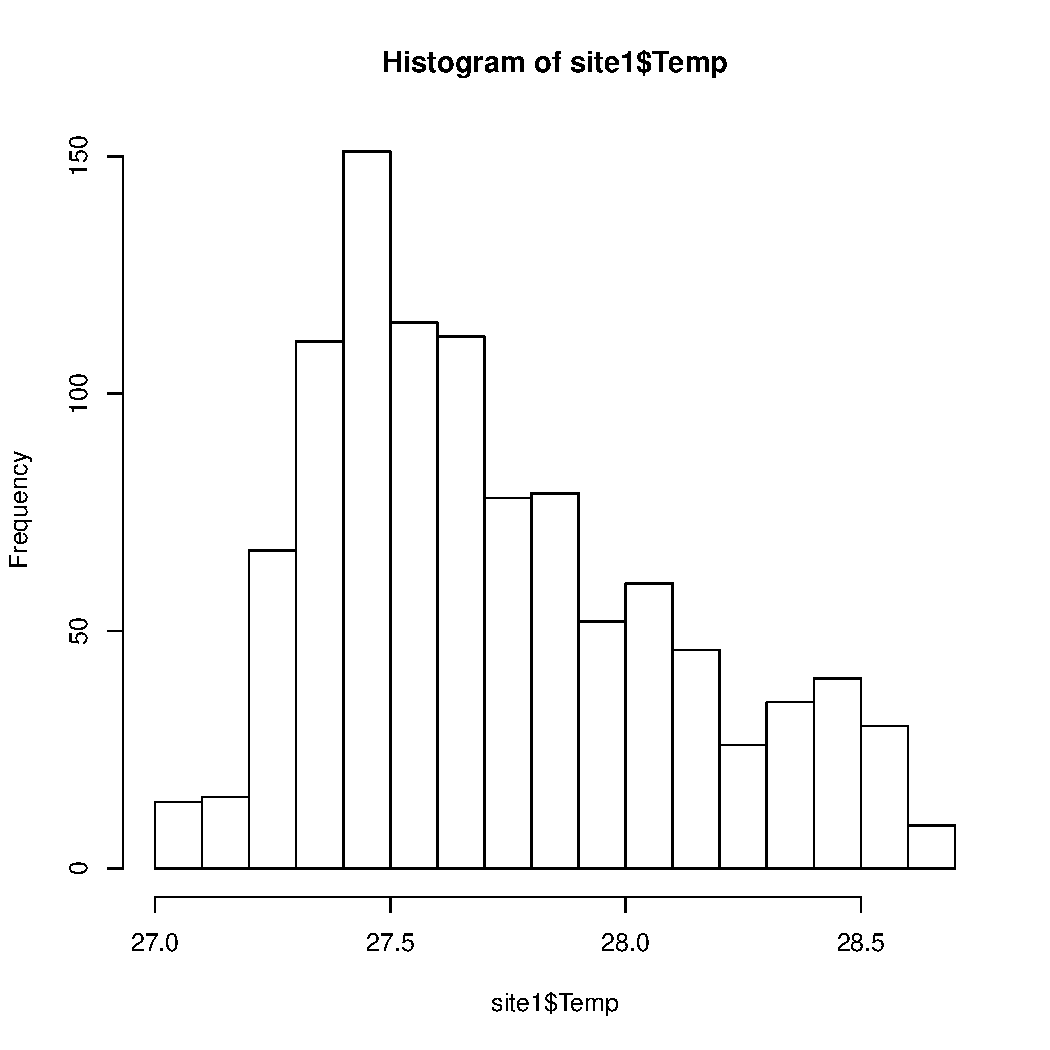
\includegraphics[width=\maxwidth]{figure/unnamed-chunk-6-1} 

\end{knitrout}

\begin{knitrout}
\definecolor{shadecolor}{rgb}{0.969, 0.969, 0.969}\color{fgcolor}\begin{kframe}
\begin{alltt}
\hlkwd{hist}\hlstd{(site2}\hlopt{$}\hlstd{Temp)}
\end{alltt}
\end{kframe}
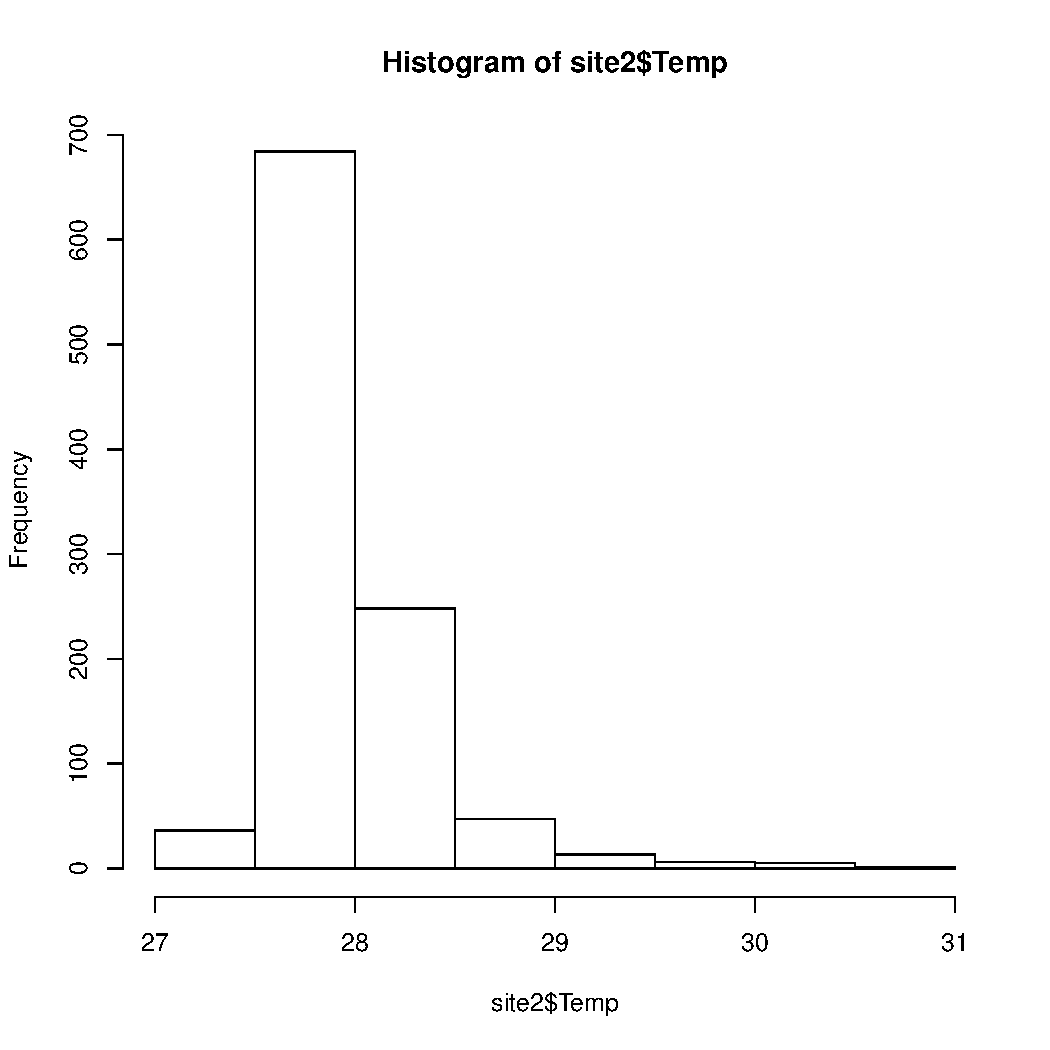
\includegraphics[width=\maxwidth]{figure/unnamed-chunk-7-1} 

\end{knitrout}

\begin{knitrout}
\definecolor{shadecolor}{rgb}{0.969, 0.969, 0.969}\color{fgcolor}\begin{kframe}
\begin{alltt}
\hlkwd{hist}\hlstd{(site3}\hlopt{$}\hlstd{Temp)}
\end{alltt}
\end{kframe}
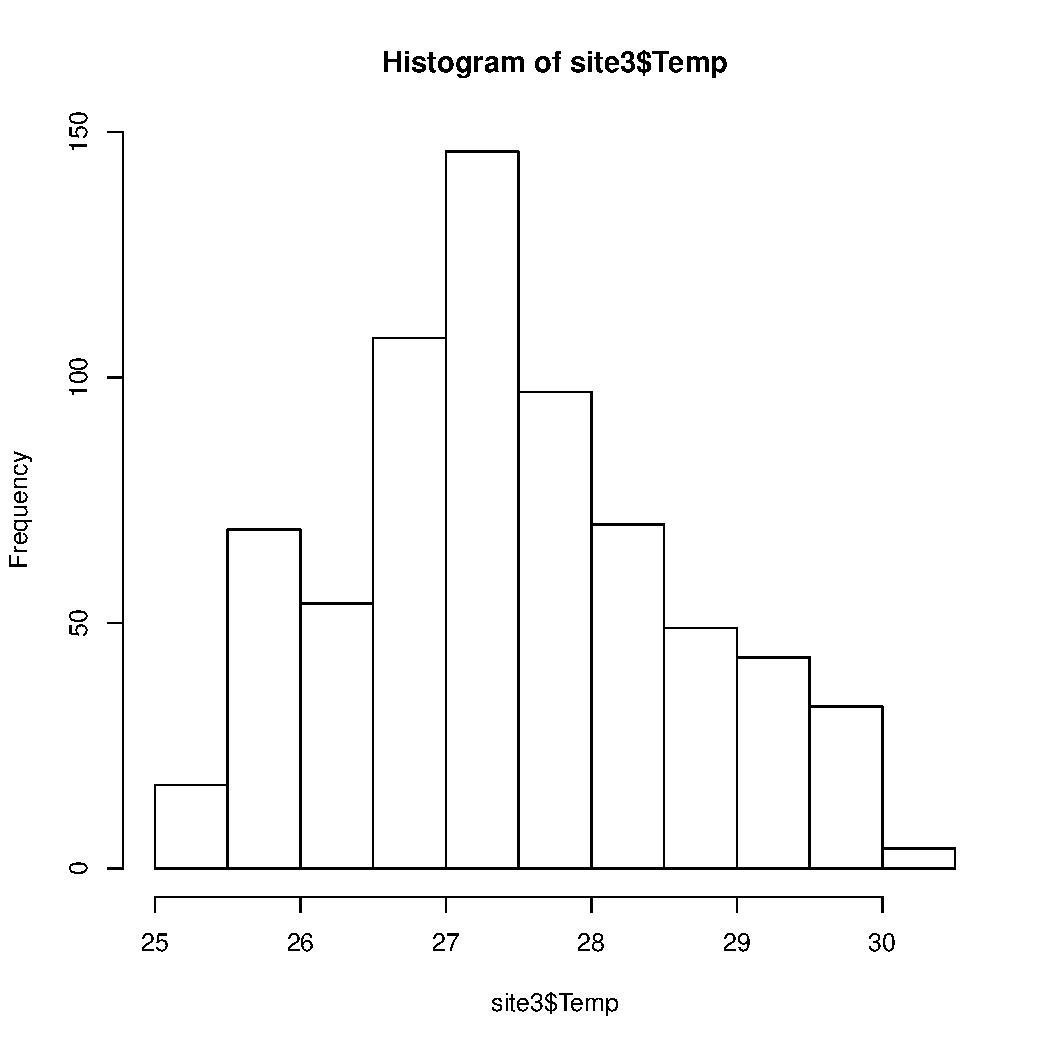
\includegraphics[width=\maxwidth]{figure/unnamed-chunk-8-1} 

\end{knitrout}

\begin{knitrout}
\definecolor{shadecolor}{rgb}{0.969, 0.969, 0.969}\color{fgcolor}\begin{kframe}
\begin{alltt}
\hlkwd{hist}\hlstd{(site4}\hlopt{$}\hlstd{Temp)}
\end{alltt}
\end{kframe}
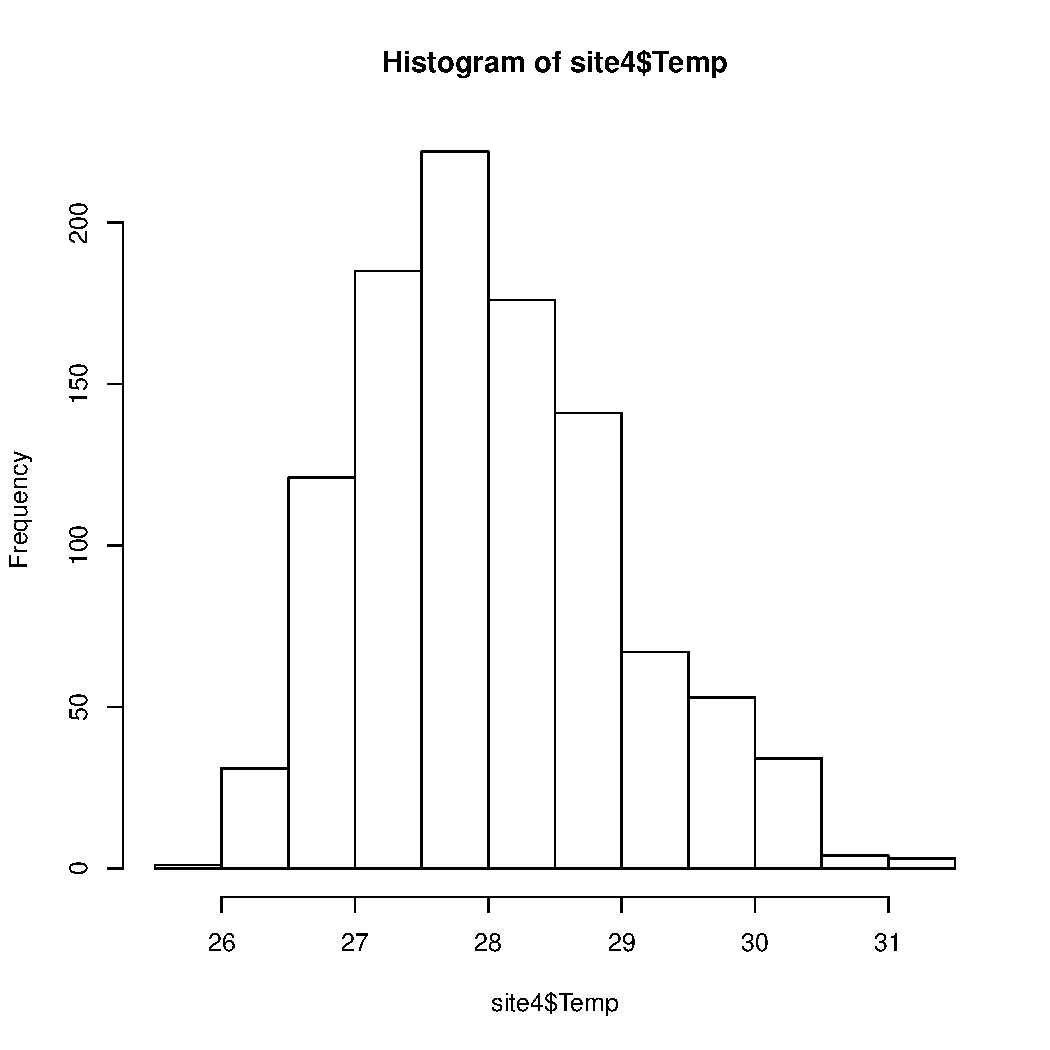
\includegraphics[width=\maxwidth]{figure/unnamed-chunk-9-1} 

\end{knitrout}

\section{Bias and Data Limitations}

Location 3 was removed four days prior to the removal of locations 1, 2, and 4. The probes also may vary in their accuracy and calibration, which will be tested for via an ice bath test. 


\end{document}
